\documentclass{standalone}
\usepackage{tikz}
\usetikzlibrary{patterns, positioning}


\begin{document}
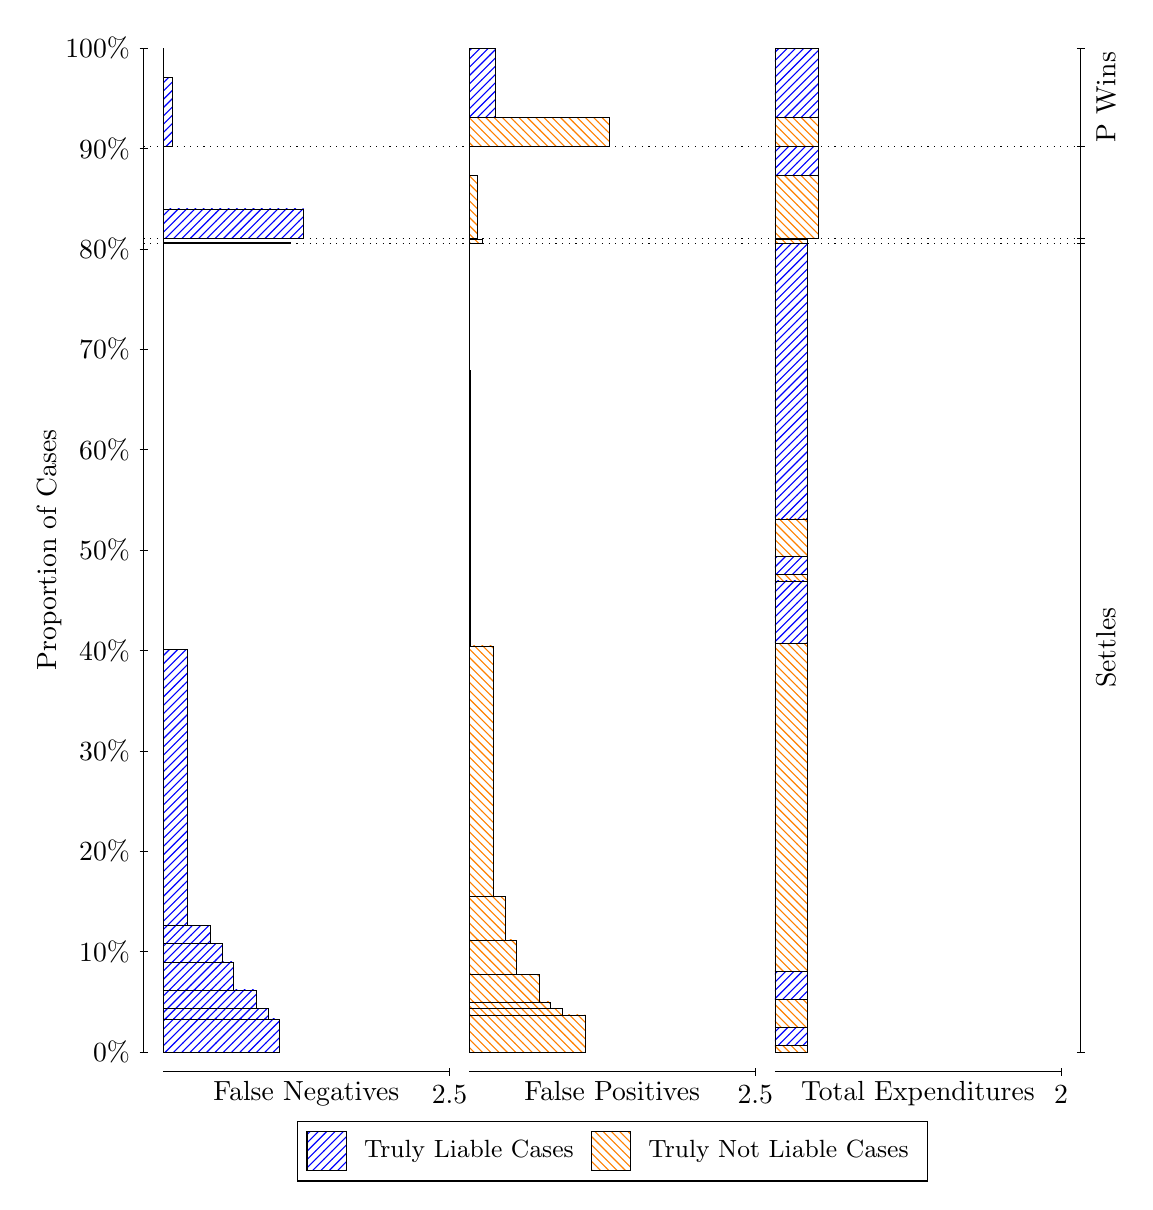
\begin{tikzpicture}
\draw[black, very thin] (1.5,1.75) -- (1.5,14.5);
\node[rotate=90, text=black, anchor=center] at (0.3, 8.125) {Proportion of Cases};
\draw[black, very thin] (1.45,1.75) -- (1.55,1.75);
\node[text=black, anchor=east] at (1.45, 1.75) {0\%};
\draw[black, very thin] (1.45,3.025) -- (1.55,3.025);
\node[text=black, anchor=east] at (1.45, 3.025) {10\%};
\draw[black, very thin] (1.45,4.3) -- (1.55,4.3);
\node[text=black, anchor=east] at (1.45, 4.3) {20\%};
\draw[black, very thin] (1.45,5.575) -- (1.55,5.575);
\node[text=black, anchor=east] at (1.45, 5.575) {30\%};
\draw[black, very thin] (1.45,6.85) -- (1.55,6.85);
\node[text=black, anchor=east] at (1.45, 6.85) {40\%};
\draw[black, very thin] (1.45,8.125) -- (1.55,8.125);
\node[text=black, anchor=east] at (1.45, 8.125) {50\%};
\draw[black, very thin] (1.45,9.4) -- (1.55,9.4);
\node[text=black, anchor=east] at (1.45, 9.4) {60\%};
\draw[black, very thin] (1.45,10.675) -- (1.55,10.675);
\node[text=black, anchor=east] at (1.45, 10.675) {70\%};
\draw[black, very thin] (1.45,11.95) -- (1.55,11.95);
\node[text=black, anchor=east] at (1.45, 11.95) {80\%};
\draw[black, very thin] (1.45,13.225) -- (1.55,13.225);
\node[text=black, anchor=east] at (1.45, 13.225) {90\%};
\draw[black, very thin] (1.45,14.5) -- (1.55,14.5);
\node[text=black, anchor=east] at (1.45, 14.5) {100\%};

\draw[black, very thin] (13.4,1.75) -- (13.4,14.5);
\draw[black, very thin] (13.35,1.75) -- (13.45,1.75);
\node[anchor=west] at (13.35, 1.75) {};
\draw[black, very thin] (13.35,12.017) -- (13.45,12.017);
\node[anchor=west] at (13.35, 12.017) {};
\draw[black, very thin] (13.35,12.085) -- (13.45,12.085);
\node[anchor=west] at (13.35, 12.085) {};
\draw[black, very thin] (13.35,13.25) -- (13.45,13.25);
\node[anchor=west] at (13.35, 13.25) {};
\draw[black, very thin] (13.35,14.5) -- (13.45,14.5);
\node[anchor=west] at (13.35, 14.5) {};

\draw[black, very thin, pattern color=blue, pattern=north east lines] (1.75,1.75) rectangle (3.2215,2.1708);
\draw[black, very thin, pattern color=blue, pattern=north east lines] (1.75,2.1708) rectangle (3.0762,2.3031);
\draw[black, very thin, pattern color=blue, pattern=north east lines] (1.75,2.3031) rectangle (2.9308,2.5391);
\draw[black, very thin, pattern color=blue, pattern=north east lines] (1.75,2.5391) rectangle (2.6402,2.8934);
\draw[black, very thin, pattern color=blue, pattern=north east lines] (1.75,2.8934) rectangle (2.4948,3.1277);
\draw[black, very thin, pattern color=blue, pattern=north east lines] (1.75,3.1277) rectangle (2.3495,3.362);
\draw[black, very thin, pattern color=blue, pattern=north east lines] (1.75,3.362) rectangle (2.0588,6.86);
\draw[black, very thin, pattern color=orange, pattern=north west lines] (1.75,6.86) rectangle (1.75,12.017);
\draw[black, very thin, pattern color=blue, pattern=north east lines] (1.75,12.017) rectangle (3.3668,12.032);
\draw[black, very thin, pattern color=orange, pattern=north west lines] (1.75,12.032) rectangle (1.75,12.085);
\draw[black, very thin, pattern color=blue, pattern=north east lines] (1.75,12.085) rectangle (3.5303,12.457);
\draw[black, very thin, pattern color=orange, pattern=north west lines] (1.75,12.457) rectangle (1.75,13.25);
\draw[black, very thin, pattern color=blue, pattern=north east lines] (1.75,13.25) rectangle (1.859,14.128);
\draw[black, very thin, pattern color=orange, pattern=north west lines] (1.75,14.128) rectangle (1.75,14.5);
\draw[black, very thin, pattern color=orange, pattern=north west lines] (5.6333,1.75) rectangle (7.1048,2.2209);
\draw[black, very thin, pattern color=orange, pattern=north west lines] (5.6333,2.2209) rectangle (6.8142,2.3031);
\draw[black, very thin, pattern color=orange, pattern=north west lines] (5.6333,2.3031) rectangle (6.6688,2.3852);
\draw[black, very thin, pattern color=orange, pattern=north west lines] (5.6333,2.3852) rectangle (6.5235,2.7396);
\draw[black, very thin, pattern color=orange, pattern=north west lines] (5.6333,2.7396) rectangle (6.2328,3.1745);
\draw[black, very thin, pattern color=orange, pattern=north west lines] (5.6333,3.1745) rectangle (6.0875,3.7259);
\draw[black, very thin, pattern color=orange, pattern=north west lines] (5.6333,3.7259) rectangle (5.9422,6.9069);
\draw[black, very thin, pattern color=blue, pattern=north east lines] (5.6333,6.9069) rectangle (5.6515,10.405);
\draw[black, very thin, pattern color=blue, pattern=north east lines] (5.6333,10.405) rectangle (5.6333,12.017);
\draw[black, very thin, pattern color=orange, pattern=north west lines] (5.6333,12.017) rectangle (5.7968,12.07);
\draw[black, very thin, pattern color=blue, pattern=north east lines] (5.6333,12.07) rectangle (5.6333,12.085);
\draw[black, very thin, pattern color=orange, pattern=north west lines] (5.6333,12.085) rectangle (5.7423,12.879);
\draw[black, very thin, pattern color=blue, pattern=north east lines] (5.6333,12.879) rectangle (5.6333,13.25);
\draw[black, very thin, pattern color=orange, pattern=north west lines] (5.6333,13.25) rectangle (7.4137,13.622);
\draw[black, very thin, pattern color=blue, pattern=north east lines] (5.6333,13.622) rectangle (5.9603,14.5);
\draw[black, very thin, pattern color=orange, pattern=north west lines] (9.5167,1.75) rectangle (9.9254,1.8322);
\draw[black, very thin, pattern color=blue, pattern=north east lines] (9.5167,1.8322) rectangle (9.9254,2.0664);
\draw[black, very thin, pattern color=orange, pattern=north west lines] (9.5167,2.0664) rectangle (9.9254,2.4208);
\draw[black, very thin, pattern color=blue, pattern=north east lines] (9.5167,2.4208) rectangle (9.9254,2.7751);
\draw[black, very thin, pattern color=orange, pattern=north west lines] (9.5167,2.7751) rectangle (9.9254,6.9425);
\draw[black, very thin, pattern color=blue, pattern=north east lines] (9.5167,6.9425) rectangle (9.9254,7.7316);
\draw[black, very thin, pattern color=orange, pattern=north west lines] (9.5167,7.7316) rectangle (9.9254,7.8137);
\draw[black, very thin, pattern color=blue, pattern=north east lines] (9.5167,7.8137) rectangle (9.9254,8.048);
\draw[black, very thin, pattern color=orange, pattern=north west lines] (9.5167,8.048) rectangle (9.9254,8.5189);
\draw[black, very thin, pattern color=blue, pattern=north east lines] (9.5167,8.5189) rectangle (9.9254,12.017);
\draw[black, very thin, pattern color=orange, pattern=north west lines] (9.5167,12.017) rectangle (9.9254,12.07);
\draw[black, very thin, pattern color=blue, pattern=north east lines] (9.5167,12.07) rectangle (9.9254,12.085);
\draw[black, very thin, pattern color=orange, pattern=north west lines] (9.5167,12.085) rectangle (10.062,12.879);
\draw[black, very thin, pattern color=blue, pattern=north east lines] (9.5167,12.879) rectangle (10.062,13.25);
\draw[black, very thin, pattern color=orange, pattern=north west lines] (9.5167,13.25) rectangle (10.062,13.622);
\draw[black, very thin, pattern color=blue, pattern=north east lines] (9.5167,13.622) rectangle (10.062,14.5);
\draw[black, dotted] (1.5,12.017) -- (13.4,12.017);
\draw[black, dotted] (1.5,12.085) -- (13.4,12.085);
\draw[black, dotted] (1.5,13.25) -- (13.4,13.25);
\draw[black, very thin] (1.75,1.5) -- (5.3833,1.5);
\node[text=black, anchor=north] at (3.5667, 1.5) {False Negatives};
\draw[black, very thin] (5.3833,1.45) -- (5.3833,1.55);
\node[text=black, anchor=north] at (5.3833, 1.45) {2.5};

\draw[black, very thin] (5.6333,1.5) -- (9.2667,1.5);
\node[text=black, anchor=north] at (7.45, 1.5) {False Positives};
\draw[black, very thin] (9.2667,1.45) -- (9.2667,1.55);
\node[text=black, anchor=north] at (9.2667, 1.45) {2.5};

\draw[black, very thin] (9.5167,1.5) -- (13.15,1.5);
\node[text=black, anchor=north] at (11.333, 1.5) {Total Expenditures};
\draw[black, very thin] (13.15,1.45) -- (13.15,1.55);
\node[text=black, anchor=north] at (13.15, 1.45) {2};

\node[text=black, centered, rotate=90] at (13.72, 6.8834) {Settles};


\node[text=black, centered, rotate=90] at (13.72, 13.875) {P Wins};

\draw (7.449999999999999,1.5) node[draw=none] (baseCoordinate) {};
\begin{scope}[align=center]
        \matrix[scale=0.5, draw=black, below=0.5cm of baseCoordinate, nodes={draw}, column sep=0.1cm]{
            \node[rectangle, draw, minimum width=0.5cm, minimum height=0.5cm, pattern color=blue, pattern=north east lines] {}; &
            \node[draw=none, font=\small, text=black] (B) {Truly Liable Cases}; &
            \node[rectangle, draw, minimum width=0.5cm, minimum height=0.5cm, pattern color=orange, pattern=north west lines] {}; &
            \node[draw=none, font=\small, text=black] (B) {Truly Not Liable Cases}; \\
            };
\end{scope}

\end{tikzpicture}
\end{document}